
\begin{frame}
\frametitle{Dirac revisited}
In modern QED we interpret the solutions of the Dirac equation as a 4-dimensional spinor $\psi$:
\[
\psi = \mqty(\psi_1 \\ \psi_2 \\ \psi_2 \\ \psi_4) = \mqty(\phi \\ \chi)
\]
where $\phi =  \mqty(\phi_1 \\ \phi_2)$ represents a particle (with two spin states) and
$\chi =  \mqty(\chi_1 \\ \chi_2)$ represents an antiparticle (also with two spin states).

Notice also that the four $\gamma$~matrices, found before, are not unique. Any set that satisfy the anticommutation relations (Clifford algebra) can be used:

\begin{empheq}[box=\fbox]{align}
\{\gamma^\mu, \gamma^\nu\} = 2 g^{\mu\nu} \nonumber
\end{empheq}

\end{frame}

\begin{frame}
\frametitle{Dirac equation using Weyl representation of the $\gamma$~matrices}
\[
\gamma^0  = \mqty(0 & I \\ I & 0),\,\,\, \gamma^i  = \mqty(0 & -\sigma^i \\ \sigma^i  & 0)
\]
Then the Dirac equation becomes:
\[
\left[ E  \mqty(0 & I \\ I & 0) - \mqty(0 & -\va{p}\cdot\va{\sigma} \\ \va{p}\cdot\va{\sigma}  & 0) -m \right]
 \mqty(\phi \\ \chi) = 0
\]
which solves into two equations:
 \begin{empheq}[box=\fbox]{align}
(E +  \va{p}\cdot\va{\sigma}) \chi - m \phi & = 0 \nonumber \\
(E -  \va{p}\cdot\va{\sigma}) \phi - m \chi & = 0 \nonumber
\end{empheq}

The first equation represents particles (electrons) while the second represent antiparticles (positrons). In each equation, the helicity states (left-handed and right handed) are coupled through the particle mass. Notice that we can "assign" unambiguously one solution to {\it matter} ($e^-$) and another to {\it antimatter} ($e^+$), given the fact, dictated by nature, that positrons and electrons are electrically charged particles (with opposite charges). 

\end{frame}

\begin{frame}
\frametitle{Describing electrons}

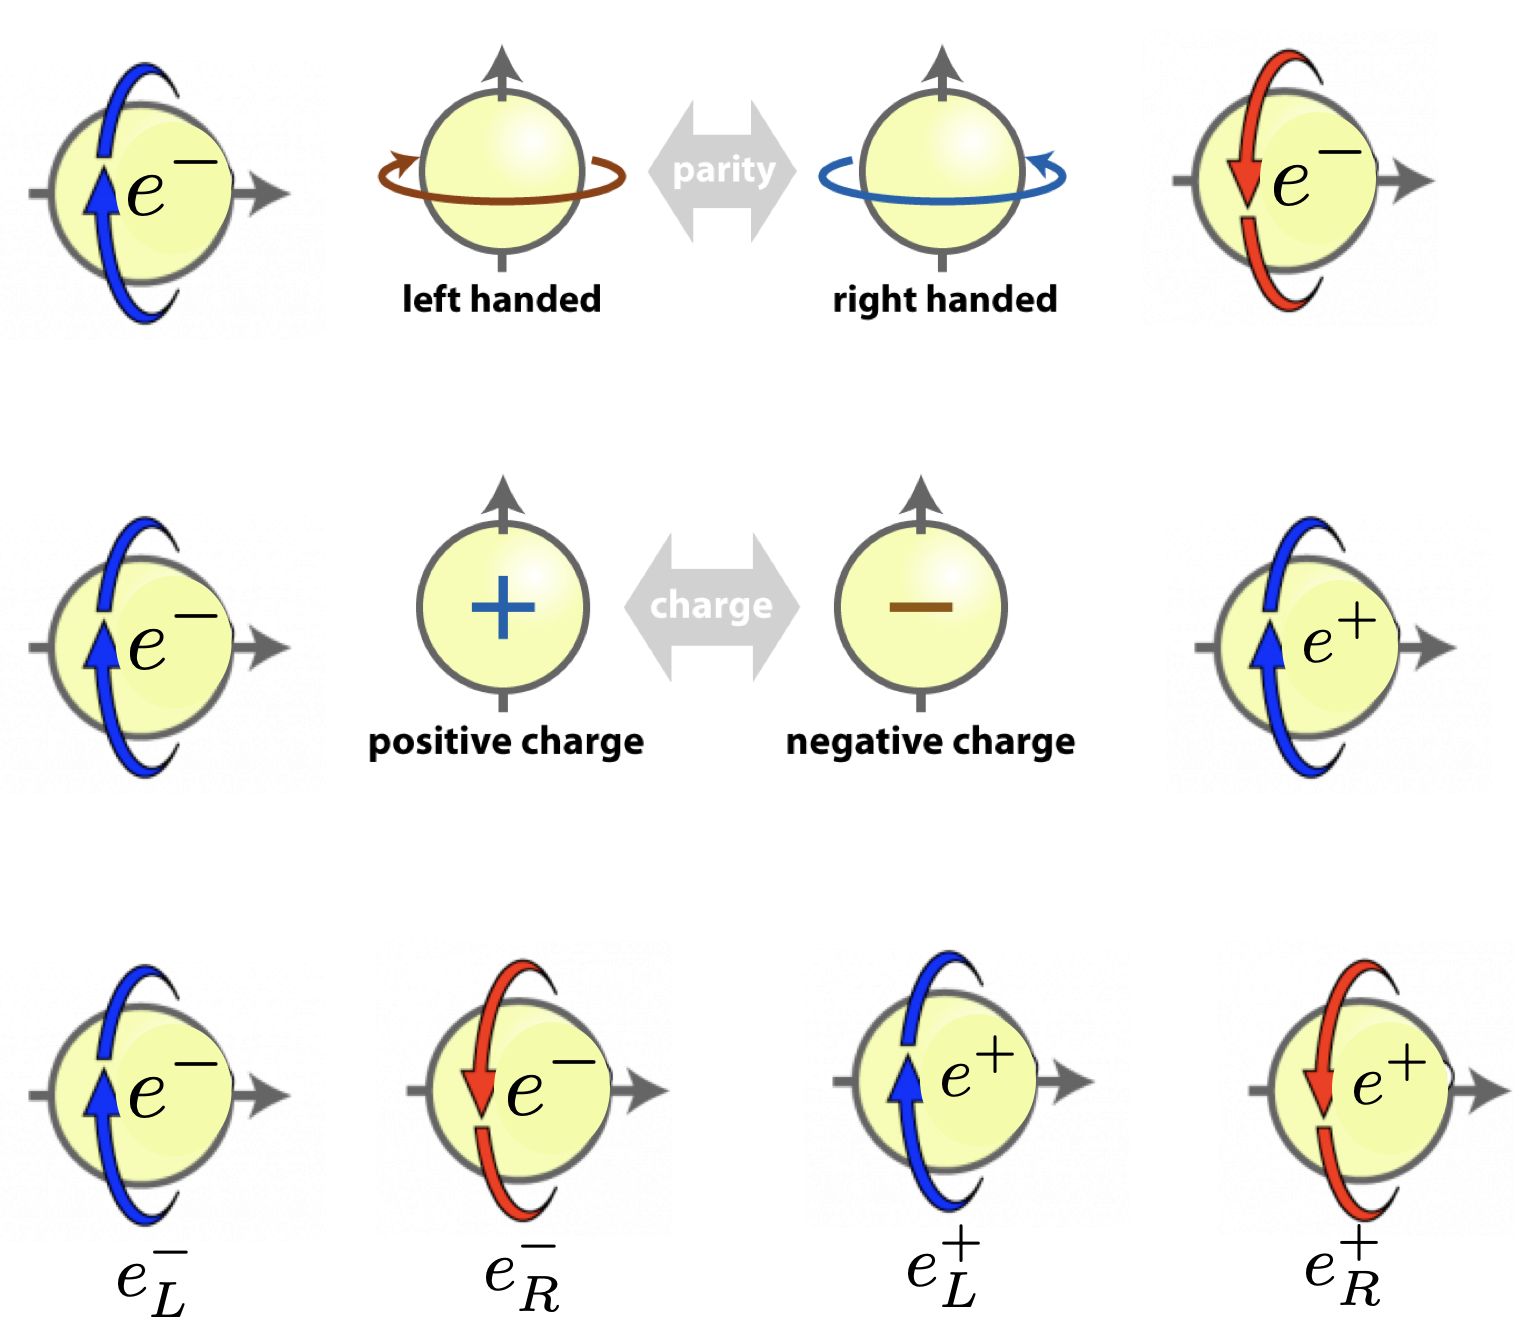
\includegraphics[scale=0.3]{img/electronsLR.png}
\end{frame}

%
%\begin{frame}
%\frametitle{Massless particles}
%In the limit of $m \rightarrow 0$~ these two equations decouple and we obtain
%two states with definite helicity:
% \begin{empheq}[box=\fbox]{align}
%(E +  \va{p}\cdot\va{\sigma}) \chi  & = 0 \nonumber \\
%(E -  \va{p}\cdot\va{\sigma}) \phi  & = 0 \nonumber
%\end{empheq}
%Notice that we have now only two degrees of freedom, since the particle has negative helicity and the antiparticle positive helicity. \alert{Massless particles have well defined helicity}. Thus, a massless $e^-$ is left-handed and a massless $e^+$ is right-handed. 
%
%\end{frame}


\begin{frame}
\frametitle{The need of Quantum Field Theory}
In spite of the heroic efforts of Dirac and others, RQM is not enough to describe elementary particles. The Dirc equation describes a single electron. Positrons need to be introduced by a sort of magical incantation (the negative sea state). In short, RQM cannot predict creation and annihilation of particles. 

Quantum Electrodynamics (QED) was eventually developed as the first Quantum Field Theory (QFT), capable of describing such creation and annihilation of particles. In QED, it is not only the photons that are quanta of a field but also the charged particles, like the electrons and positrons. The fields are operators that create and annihilate their quanta. \alert{Thus $\psi(x)$~is no longer interpreted as a waveform that describes probability but as an operator that creates a particle in point $x$~and destroys an antiparticle in $x$ ($\bar{\psi}(x)$~will create an antiparticle in point $x$~and destroy antiparticle in $x$)}.

The Lagrangian of the free Dirac field $\psi$~is given by:

\begin{empheq}[box=\fbox]{align}
  L = \bar{\psi}(i\gamma^\mu \partial_\mu -m)\psi  \nonumber
\end{empheq}

where $\bar{\psi} = \psi^\dagger \gamma^0$. Varying the Lagrangian yields back the Dirac equation. 
%The $\gamma$~matrices found by Dirac were complex. This means that the spinor field $\psi$~must also be complex. This makes sense from the point of view of field theory as a complex field would create particles and annihilate anti-particles while its complex conjugate would create anti-particles and annihilate particles. However, as we shall see, Majorana found an alternative. 

\end{frame}


\begin{frame}
\frametitle{Feynman Diagrams}
\begin{columns}
\column{0.4\textwidth}
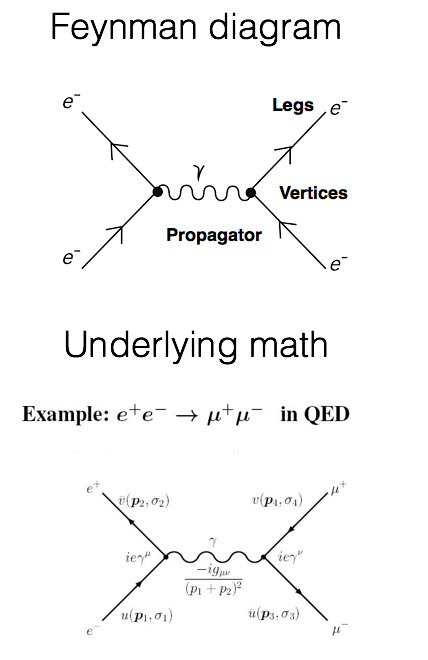
\includegraphics[scale=0.3]{img/FeynmanD2.png}
 
\column{0.5\textwidth}
Feynman diagrams: ``pictures'' whose lines are world-lines of the particles in the space-time. They are representations of mathematical expressions of scattering or decay amplitudes. We cannot do the math here, but the diagrams suggest nicely the underlying physics. 

\end{columns}
\end{frame}
\begin{frame}
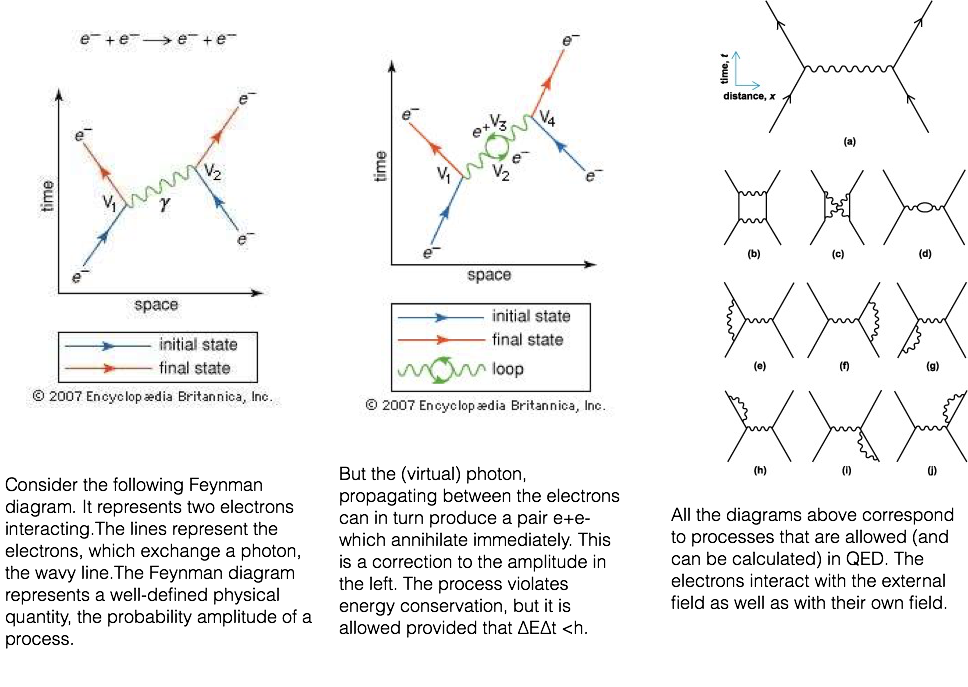
\includegraphics[scale=0.3]{img/FeynmanD3.png}

\end{frame}